\documentclass[12pt, a4paper, twocolumn]{article}

\usepackage[utf8]{inputenc}
\usepackage[T1]{fontenc}
\usepackage[english]{babel}
\usepackage{lmodern}
\usepackage{geometry}
\usepackage{hyperref}
\usepackage[dvipsnames]{xcolor}
\usepackage[bf,sf,small,pagestyles]{titlesec}
\usepackage{titling}
\usepackage{abstract}
\usepackage[font={footnotesize, sf}, labelfont=bf]{caption} 
\usepackage{siunitx}
\usepackage{graphicx}
\usepackage{booktabs}
\usepackage{amsmath,amssymb}
\usepackage{physics}
\usepackage[sort]{cleveref}
\usepackage{enumitem}
\usepackage{bibtopic}
\usepackage{chemformula}

\geometry{
	a4paper,
	right = 2.5cm,
	left = 2.5cm,
	bottom = 3cm,
	top = 3cm
}

\hypersetup{
	colorlinks,
	linkcolor = {red!50!blue},
	citecolor = {red!50!blue},
	linktoc = page
}

\numberwithin{table}{section}
\numberwithin{figure}{section}
\numberwithin{equation}{section}

\graphicspath{{./figs/}}

% Unitats
\sisetup{
	inter-unit-product = \ensuremath{ \, },
	allow-number-unit-breaks = true,
	detect-family = true,
	list-units = single,
	math-celsius = {}^{\circ}\kern-\scriptspace C
}

\DeclareMathAlphabet{\mathsfit}{T1}{\sfdefault}{\mddefault}{\sldefault}

\newcommand{\Z}{\mathbb{Z}}
\renewcommand{\vec}[1]{\mathbf{#1}}
\newcommand{\N}{\mathbb{N}}
\newcommand{\R}{\mathbb{R}}
\newcommand{\Ry}{\mathit{Ry}}
\newcommand{\inn}[2]{\left\langle #1 , #2 \right\rangle}
\newcommand{\proj}[1]{\ketbra{#1}{#1}}
\newcommand{\parbreak}{
	\begin{center}
		--- $\ast$ ---
	\end{center} 
}
\makeatletter
\newcommand*{\defeq}{\mathrel{\rlap{%
    \raisebox{0.3ex}{$\m@th\cdot$}}%
  \raisebox{-0.3ex}{$\m@th\cdot$}}%
=
}
\makeatother

\newpagestyle{pagina}{
	\headrule
	\sethead*{\bfseries \sffamily Compost Pile Sizes}{}{\theauthor}
	\footrule
	\setfoot*{}{}{\sffamily \thepage}
}
\renewpagestyle{plain}{
	\footrule
	\setfoot*{}{}{\sffamily \thepage}
}
\pagestyle{pagina}

\title{\sffamily \bfseries Problem B: Compost Pile Sizes}
\author{\sffamily Team 242}
\date{}

\begin{document}
\renewcommand{\abstractname}{}
\renewcommand{\absnamepos}{empty}
\begin{titlingpage}
 \maketitle

\noindent \hrulefill \\
\begin{abstract}
The aim of this report is to discuss the viability of a solar sail mission to Mars. Results have been obtained by attempting to solve the equations that govern the motion of a solar sail in the Solar System. Under suitable approximations, these are analytically solvable. The general case, however, is not, and required the use of numerical techniques. 

Results show such a mission would be indeed feasible, allowing for payloads of \SI{1000}{kg} to be sent to Mars' orbit within about a year. However, actual arrival to Mars, subject to the required initial conditions, has been found to be of high complexity. In spite of this, some trajectories have been found that bring the craft close enough to Mars at the cost of a higher, even if still reasonable, travel time. Additionally, with the introduction of a simple steering maneuver, it has been found that it is possible for the solar sail to reach the orbit of Mars and to remain stable in it for a sufficiently long timescale.

All of these results seem to suggest that solar sailing is indeed a suitable method of light inner Solar System travel, especially given its simplicity when compared to the other more common options. 
\end{abstract}
\hrulefill
\end{titlingpage}

\begin{titlingpage}
\tableofcontents
\end{titlingpage}

\section{Introduction}
\cite{mason}

\section{The composting process}
\subsection{History and relevancy of composting}
Composting is defined as the biological oxidative decomposition of organic constituents in wastes (generally organic) under controlled conditions.
\subsection{Phases of the process}
During the process of composting, the substrate evolves through three principal phases:

\textbf{Mesophilic phase:} In the first stage, mesophilic microbes proliferate rapidly in the organic matter and decompose readily degradable components, such as sugars. This process releases heat and lasts between one and five days, when the temperature raises up to \SI{40}{\celsius} and this type of microbes become increasingly inhibited.

\textbf{Thermophilic phase:} The raise in temperature activates the thermophilic microbes, which decompose cellulose, protein and fats. This biooxidative activity produces \ch{CO2} and \ch{H2O} and realeses a lot of heat. This part of the process is important because the high temperatures destroy animal and plant pathogens.

\textbf{Maturation and "curing" phase:} As microbial populations stabilize, decomposition rate decreases and temperature declines, allowing mesophilic microorganisms to recolonize the compost. A process of stabilization and mineralization where the most stable organic compounds are decomposed and the compost becomes a "humified" final product.
 
\subsubsection{Mesophilic and thermophilic microbes}
\subsection{Physical factors}


\section{Model}

\subsection{Theoretical model}

\subsubsection{Environment}

The compost pile will be exposed to day-night temperature shift, since it will be left outdoors. Thus, we will consider a varying room temperature between \SI{5}{\celsius} and \si{20}{\celsius} as a sinusoidal function for our pile. In addition, we will let the leftovers begin at a \SI{20}{\celsius} temperature.  

\subsubsection{Compost}

We are trying to study the decomposition of kitchen vegetable waste, and hence we will not produce a big amount of compost. For a medium-size family, \si{30}{kg} seems an adequate monthly output of organic waste. 

For the sake of simplicity, we can assume that our pile will be homogeneous: we will mix the pile initially in a way such that we are not able to distinguish the solid, liquid and gas phase. This way we can also assume that the thermophysical properties will remain constant, including the porosity. (It might be thought that as the decomposition goes on, the gas phase will grow bigger and therefore the porosity will be reduced, but we will consider an average value of it.) %SOBRA? 

With regard to moisture, it is widely known that its content of the composting materials diminishes due to evaporation, nonetheless if the evaporation is compensated by the water being fed with the gas phase; the moisture content could be kept nearly constant \cite{niceassumptions}. We may assume then a moisture level of a 50\%, for it is a reasonable percentage considering only vegetable kitchen waste and its high amount of water. 

Any periodic aeration of the pile will be avoided. The dimensions of the compost pile are not big enough to require an external aeration system. Due to the low thermal conductance of the container and the possibility of some slow air flow through the holes of it, the compost will receive the oxygen it needs in order to keep up with the decomposition but without having a big effect on the temperature. In case any of our designs reached high temperatures (above \si{60}{\celsius} or so), it will be discarded. 

As we were saying, the container of the pile will be thought as a HDPE cubic box not completely isolated (i.e. some air flow is permitted). This way we will avoid the lack of oxygen without losing the isolation. The walls of it will be thin, this way we can neglect the heat losses due to conduction, and will also grant a weaker isolation that will lead to smoother temperatures. 

\subsubsection{Microbes}

Our model will consist of a compost pile in which two main types of microbe produce the decomposition and release energy: mesophiles and thermophiles. We assume that the mesophilic microbes will activate at room temperature and will inactivate at \si{40}{\celsius}, where they reach their peak activity, whereas thermophilic microbes will take over at this temperature and inactivate at \si{60}{\celsius}. We also assume that the exothermicity of the first part of the decomposition is bigger than the second, so the thermophiles will present a slower growth than the others.

Our model has been based on the empirical data of the decomposition of vegetable waste produced by the mesophile \textit{aspergillus niger}\cite{mesophile}. From this information we were able to 

\subsection{Numerical model}
We will ground our model of the evolution of a compost pile on its heat balance equation. There are two main terms at play: the heat produced by the biochemical process of composting, \( \dot{Q}_c \) and the heat losses of the pile, \( \dot{Q}_l \). We can thus write
\begin{equation} \label{eq:first balance}
	\dot{Q} = \dot{Q}_c + \dot{Q}_l. 
\end{equation}
We will consider the temperature within the compost pile to be constant throughout, as well as its heat capacity, and so the first term of \cref{eq:first balance} becomes \( \dot{Q} = mc\dot{T} \), where \( m \) is the mass of the pile and \( c \) its specific heat capacity. As for the losses, given the temperature range we are considering, \SIrange{20}{70}{\celsius}, it seems reasonable to assume that these are mainly due to convection. Radiation in this range of temperatures is perfectly negligible. Thus we may write \( \dot{Q}_l = -UA\left(T - T_\text{env}\right) \), where \( U \) is the overall heat transfer coefficient, in \si{W.m^{-1}.K^{-1}}, \( A \) is the total surface area of the pile and \( T_\text{env} \) is the outside temperature. We may also discard losses due to conduction, since we consider the walls of the pile to be thin.

\begin{figure}[htb]
	\sffamily \footnotesize \centering
	% GNUPLOT: LaTeX picture with Postscript
\begingroup
  \makeatletter
  \providecommand\color[2][]{%
    \GenericError{(gnuplot) \space\space\space\@spaces}{%
      Package color not loaded in conjunction with
      terminal option `colourtext'%
    }{See the gnuplot documentation for explanation.%
    }{Either use 'blacktext' in gnuplot or load the package
      color.sty in LaTeX.}%
    \renewcommand\color[2][]{}%
  }%
  \providecommand\includegraphics[2][]{%
    \GenericError{(gnuplot) \space\space\space\@spaces}{%
      Package graphicx or graphics not loaded%
    }{See the gnuplot documentation for explanation.%
    }{The gnuplot epslatex terminal needs graphicx.sty or graphics.sty.}%
    \renewcommand\includegraphics[2][]{}%
  }%
  \providecommand\rotatebox[2]{#2}%
  \@ifundefined{ifGPcolor}{%
    \newif\ifGPcolor
    \GPcolortrue
  }{}%
  \@ifundefined{ifGPblacktext}{%
    \newif\ifGPblacktext
    \GPblacktextfalse
  }{}%
  % define a \g@addto@macro without @ in the name:
  \let\gplgaddtomacro\g@addto@macro
  % define empty templates for all commands taking text:
  \gdef\gplbacktext{}%
  \gdef\gplfronttext{}%
  \makeatother
  \ifGPblacktext
    % no textcolor at all
    \def\colorrgb#1{}%
    \def\colorgray#1{}%
  \else
    % gray or color?
    \ifGPcolor
      \def\colorrgb#1{\color[rgb]{#1}}%
      \def\colorgray#1{\color[gray]{#1}}%
      \expandafter\def\csname LTw\endcsname{\color{white}}%
      \expandafter\def\csname LTb\endcsname{\color{black}}%
      \expandafter\def\csname LTa\endcsname{\color{black}}%
      \expandafter\def\csname LT0\endcsname{\color[rgb]{1,0,0}}%
      \expandafter\def\csname LT1\endcsname{\color[rgb]{0,1,0}}%
      \expandafter\def\csname LT2\endcsname{\color[rgb]{0,0,1}}%
      \expandafter\def\csname LT3\endcsname{\color[rgb]{1,0,1}}%
      \expandafter\def\csname LT4\endcsname{\color[rgb]{0,1,1}}%
      \expandafter\def\csname LT5\endcsname{\color[rgb]{1,1,0}}%
      \expandafter\def\csname LT6\endcsname{\color[rgb]{0,0,0}}%
      \expandafter\def\csname LT7\endcsname{\color[rgb]{1,0.3,0}}%
      \expandafter\def\csname LT8\endcsname{\color[rgb]{0.5,0.5,0.5}}%
    \else
      % gray
      \def\colorrgb#1{\color{black}}%
      \def\colorgray#1{\color[gray]{#1}}%
      \expandafter\def\csname LTw\endcsname{\color{white}}%
      \expandafter\def\csname LTb\endcsname{\color{black}}%
      \expandafter\def\csname LTa\endcsname{\color{black}}%
      \expandafter\def\csname LT0\endcsname{\color{black}}%
      \expandafter\def\csname LT1\endcsname{\color{black}}%
      \expandafter\def\csname LT2\endcsname{\color{black}}%
      \expandafter\def\csname LT3\endcsname{\color{black}}%
      \expandafter\def\csname LT4\endcsname{\color{black}}%
      \expandafter\def\csname LT5\endcsname{\color{black}}%
      \expandafter\def\csname LT6\endcsname{\color{black}}%
      \expandafter\def\csname LT7\endcsname{\color{black}}%
      \expandafter\def\csname LT8\endcsname{\color{black}}%
    \fi
  \fi
    \setlength{\unitlength}{0.0500bp}%
    \ifx\gptboxheight\undefined%
      \newlength{\gptboxheight}%
      \newlength{\gptboxwidth}%
      \newsavebox{\gptboxtext}%
    \fi%
    \setlength{\fboxrule}{0.5pt}%
    \setlength{\fboxsep}{1pt}%
\begin{picture}(4420.00,3400.00)%
    \gplgaddtomacro\gplbacktext{%
      \csname LTb\endcsname%%
      \put(420,380){\makebox(0,0)[r]{\strut{}\num{10}}}%
      \csname LTb\endcsname%%
      \put(420,702){\makebox(0,0)[r]{\strut{}\num{15}}}%
      \csname LTb\endcsname%%
      \put(420,1024){\makebox(0,0)[r]{\strut{}\num{20}}}%
      \csname LTb\endcsname%%
      \put(420,1347){\makebox(0,0)[r]{\strut{}\num{25}}}%
      \csname LTb\endcsname%%
      \put(420,1669){\makebox(0,0)[r]{\strut{}\num{30}}}%
      \csname LTb\endcsname%%
      \put(420,1991){\makebox(0,0)[r]{\strut{}\num{35}}}%
      \csname LTb\endcsname%%
      \put(420,2313){\makebox(0,0)[r]{\strut{}\num{40}}}%
      \csname LTb\endcsname%%
      \put(420,2636){\makebox(0,0)[r]{\strut{}\num{45}}}%
      \csname LTb\endcsname%%
      \put(420,2958){\makebox(0,0)[r]{\strut{}\num{50}}}%
      \csname LTb\endcsname%%
      \put(420,3280){\makebox(0,0)[r]{\strut{}\num{55}}}%
      \csname LTb\endcsname%%
      \put(487,261){\makebox(0,0){\strut{}\num{0}}}%
      \csname LTb\endcsname%%
      \put(1089,261){\makebox(0,0){\strut{}\num{5}}}%
      \csname LTb\endcsname%%
      \put(1691,261){\makebox(0,0){\strut{}\num{10}}}%
      \csname LTb\endcsname%%
      \put(2292,261){\makebox(0,0){\strut{}\num{15}}}%
      \csname LTb\endcsname%%
      \put(2894,261){\makebox(0,0){\strut{}\num{20}}}%
      \csname LTb\endcsname%%
      \put(3496,261){\makebox(0,0){\strut{}\num{25}}}%
      \csname LTb\endcsname%%
      \put(4098,261){\makebox(0,0){\strut{}\num{30}}}%
    }%
    \gplgaddtomacro\gplfronttext{%
      \csname LTb\endcsname%%
      \put(100,1830){\rotatebox{-270}{\makebox(0,0){\strut{}$\mathsfit T \ (\si{\celsius})$}}}%
      \csname LTb\endcsname%%
      \put(2352,83){\makebox(0,0){\strut{}$\mathsfit t \ (\si{days})$}}%
    }%
    \gplbacktext
    \put(0,0){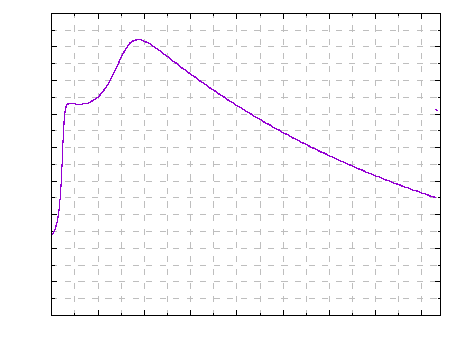
\includegraphics{2-temperatura}}%
    \gplfronttext
  \end{picture}%
\endgroup

	\caption{Temperature evolution of the compost pile modeled with mesophilic and thermophilic populations}
	\label{fig:temp-mesos-termos}
\end{figure}

\begin{figure}[htb]
	\sffamily \footnotesize \centering
	% GNUPLOT: LaTeX picture with Postscript
\begingroup
\newcommand{\etiqueta}[1]{\setlength{\fboxsep}{0.75pt}\colorbox{white}{#1}}
  \makeatletter
  \providecommand\color[2][]{%
    \GenericError{(gnuplot) \space\space\space\@spaces}{%
      Package color not loaded in conjunction with
      terminal option `colourtext'%
    }{See the gnuplot documentation for explanation.%
    }{Either use 'blacktext' in gnuplot or load the package
      color.sty in LaTeX.}%
    \renewcommand\color[2][]{}%
  }%
  \providecommand\includegraphics[2][]{%
    \GenericError{(gnuplot) \space\space\space\@spaces}{%
      Package graphicx or graphics not loaded%
    }{See the gnuplot documentation for explanation.%
    }{The gnuplot epslatex terminal needs graphicx.sty or graphics.sty.}%
    \renewcommand\includegraphics[2][]{}%
  }%
  \providecommand\rotatebox[2]{#2}%
  \@ifundefined{ifGPcolor}{%
    \newif\ifGPcolor
    \GPcolortrue
  }{}%
  \@ifundefined{ifGPblacktext}{%
    \newif\ifGPblacktext
    \GPblacktextfalse
  }{}%
  % define a \g@addto@macro without @ in the name:
  \let\gplgaddtomacro\g@addto@macro
  % define empty templates for all commands taking text:
  \gdef\gplbacktext{}%
  \gdef\gplfronttext{}%
  \makeatother
  \ifGPblacktext
    % no textcolor at all
    \def\colorrgb#1{}%
    \def\colorgray#1{}%
  \else
    % gray or color?
    \ifGPcolor
      \def\colorrgb#1{\color[rgb]{#1}}%
      \def\colorgray#1{\color[gray]{#1}}%
      \expandafter\def\csname LTw\endcsname{\color{white}}%
      \expandafter\def\csname LTb\endcsname{\color{black}}%
      \expandafter\def\csname LTa\endcsname{\color{black}}%
      \expandafter\def\csname LT0\endcsname{\color[rgb]{1,0,0}}%
      \expandafter\def\csname LT1\endcsname{\color[rgb]{0,1,0}}%
      \expandafter\def\csname LT2\endcsname{\color[rgb]{0,0,1}}%
      \expandafter\def\csname LT3\endcsname{\color[rgb]{1,0,1}}%
      \expandafter\def\csname LT4\endcsname{\color[rgb]{0,1,1}}%
      \expandafter\def\csname LT5\endcsname{\color[rgb]{1,1,0}}%
      \expandafter\def\csname LT6\endcsname{\color[rgb]{0,0,0}}%
      \expandafter\def\csname LT7\endcsname{\color[rgb]{1,0.3,0}}%
      \expandafter\def\csname LT8\endcsname{\color[rgb]{0.5,0.5,0.5}}%
    \else
      % gray
      \def\colorrgb#1{\color{black}}%
      \def\colorgray#1{\color[gray]{#1}}%
      \expandafter\def\csname LTw\endcsname{\color{white}}%
      \expandafter\def\csname LTb\endcsname{\color{black}}%
      \expandafter\def\csname LTa\endcsname{\color{black}}%
      \expandafter\def\csname LT0\endcsname{\color{black}}%
      \expandafter\def\csname LT1\endcsname{\color{black}}%
      \expandafter\def\csname LT2\endcsname{\color{black}}%
      \expandafter\def\csname LT3\endcsname{\color{black}}%
      \expandafter\def\csname LT4\endcsname{\color{black}}%
      \expandafter\def\csname LT5\endcsname{\color{black}}%
      \expandafter\def\csname LT6\endcsname{\color{black}}%
      \expandafter\def\csname LT7\endcsname{\color{black}}%
      \expandafter\def\csname LT8\endcsname{\color{black}}%
    \fi
  \fi
    \setlength{\unitlength}{0.0500bp}%
    \ifx\gptboxheight\undefined%
      \newlength{\gptboxheight}%
      \newlength{\gptboxwidth}%
      \newsavebox{\gptboxtext}%
    \fi%
    \setlength{\fboxrule}{0.5pt}%
    \setlength{\fboxsep}{1pt}%
\begin{picture}(4420.00,3400.00)%
    \gplgaddtomacro\gplbacktext{%
      \csname LTb\endcsname%%
      \put(420,380){\makebox(0,0)[r]{\strut{}\num{10}}}%
      \csname LTb\endcsname%%
      \put(420,907){\makebox(0,0)[r]{\strut{}\num{20}}}%
      \csname LTb\endcsname%%
      \put(420,1435){\makebox(0,0)[r]{\strut{}\num{30}}}%
      \csname LTb\endcsname%%
      \put(420,1962){\makebox(0,0)[r]{\strut{}\num{40}}}%
      \csname LTb\endcsname%%
      \put(420,2489){\makebox(0,0)[r]{\strut{}\num{50}}}%
      \csname LTb\endcsname%%
      \put(420,3016){\makebox(0,0)[r]{\strut{}\num{60}}}%
      \csname LTb\endcsname%%
      \put(487,261){\makebox(0,0){\strut{}\num{0}}}%
      \csname LTb\endcsname%%
      \put(1089,261){\makebox(0,0){\strut{}\num{5}}}%
      \csname LTb\endcsname%%
      \put(1691,261){\makebox(0,0){\strut{}\num{10}}}%
      \csname LTb\endcsname%%
      \put(2292,261){\makebox(0,0){\strut{}\num{15}}}%
      \csname LTb\endcsname%%
      \put(2894,261){\makebox(0,0){\strut{}\num{20}}}%
      \csname LTb\endcsname%%
      \put(3496,261){\makebox(0,0){\strut{}\num{25}}}%
      \csname LTb\endcsname%%
      \put(4098,261){\makebox(0,0){\strut{}\num{30}}}%
    }%
    \gplgaddtomacro\gplfronttext{%
      \csname LTb\endcsname%%
      \put(100,1830){\rotatebox{-270}{\makebox(0,0){\strut{}$\mathsfit T \ (\si{\celsius})$}}}%
      \csname LTb\endcsname%%
      \put(2352,83){\makebox(0,0){\strut{}$\mathsfit t \ (\si{days})$}}%
      \csname LTb\endcsname%%
      \put(3737,3069){\rotatebox{-5}{\makebox(0,0){\strut{}\etiqueta{\footnotesize $\mathsfit{A} = \SI{1}{m^2}$}}}}%
      \csname LTb\endcsname%%
      \put(2894,1487){\rotatebox{-25}{\makebox(0,0){\strut{}\etiqueta{\footnotesize $\mathsfit{A} = \SI{10}{m^2}$}}}}%
    }%
    \gplbacktext
    \put(0,0){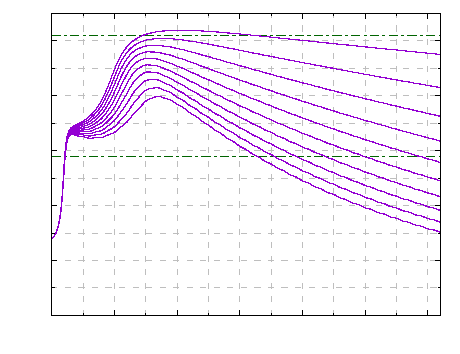
\includegraphics{2-temperatura-A}}%
    \gplfronttext
  \end{picture}%
\endgroup

	\caption{Temperature evolution of the compost pile for various values of surface area}
	\label{fig:temp-arees}
\end{figure}

\begin{figure}[htb]
	\sffamily \footnotesize \centering
	% GNUPLOT: LaTeX picture with Postscript
\begingroup
\newcommand{\etiqueta}[1]{\setlength{\fboxsep}{0.75pt}\colorbox{white}{#1}}
  \makeatletter
  \providecommand\color[2][]{%
    \GenericError{(gnuplot) \space\space\space\@spaces}{%
      Package color not loaded in conjunction with
      terminal option `colourtext'%
    }{See the gnuplot documentation for explanation.%
    }{Either use 'blacktext' in gnuplot or load the package
      color.sty in LaTeX.}%
    \renewcommand\color[2][]{}%
  }%
  \providecommand\includegraphics[2][]{%
    \GenericError{(gnuplot) \space\space\space\@spaces}{%
      Package graphicx or graphics not loaded%
    }{See the gnuplot documentation for explanation.%
    }{The gnuplot epslatex terminal needs graphicx.sty or graphics.sty.}%
    \renewcommand\includegraphics[2][]{}%
  }%
  \providecommand\rotatebox[2]{#2}%
  \@ifundefined{ifGPcolor}{%
    \newif\ifGPcolor
    \GPcolortrue
  }{}%
  \@ifundefined{ifGPblacktext}{%
    \newif\ifGPblacktext
    \GPblacktextfalse
  }{}%
  % define a \g@addto@macro without @ in the name:
  \let\gplgaddtomacro\g@addto@macro
  % define empty templates for all commands taking text:
  \gdef\gplbacktext{}%
  \gdef\gplfronttext{}%
  \makeatother
  \ifGPblacktext
    % no textcolor at all
    \def\colorrgb#1{}%
    \def\colorgray#1{}%
  \else
    % gray or color?
    \ifGPcolor
      \def\colorrgb#1{\color[rgb]{#1}}%
      \def\colorgray#1{\color[gray]{#1}}%
      \expandafter\def\csname LTw\endcsname{\color{white}}%
      \expandafter\def\csname LTb\endcsname{\color{black}}%
      \expandafter\def\csname LTa\endcsname{\color{black}}%
      \expandafter\def\csname LT0\endcsname{\color[rgb]{1,0,0}}%
      \expandafter\def\csname LT1\endcsname{\color[rgb]{0,1,0}}%
      \expandafter\def\csname LT2\endcsname{\color[rgb]{0,0,1}}%
      \expandafter\def\csname LT3\endcsname{\color[rgb]{1,0,1}}%
      \expandafter\def\csname LT4\endcsname{\color[rgb]{0,1,1}}%
      \expandafter\def\csname LT5\endcsname{\color[rgb]{1,1,0}}%
      \expandafter\def\csname LT6\endcsname{\color[rgb]{0,0,0}}%
      \expandafter\def\csname LT7\endcsname{\color[rgb]{1,0.3,0}}%
      \expandafter\def\csname LT8\endcsname{\color[rgb]{0.5,0.5,0.5}}%
    \else
      % gray
      \def\colorrgb#1{\color{black}}%
      \def\colorgray#1{\color[gray]{#1}}%
      \expandafter\def\csname LTw\endcsname{\color{white}}%
      \expandafter\def\csname LTb\endcsname{\color{black}}%
      \expandafter\def\csname LTa\endcsname{\color{black}}%
      \expandafter\def\csname LT0\endcsname{\color{black}}%
      \expandafter\def\csname LT1\endcsname{\color{black}}%
      \expandafter\def\csname LT2\endcsname{\color{black}}%
      \expandafter\def\csname LT3\endcsname{\color{black}}%
      \expandafter\def\csname LT4\endcsname{\color{black}}%
      \expandafter\def\csname LT5\endcsname{\color{black}}%
      \expandafter\def\csname LT6\endcsname{\color{black}}%
      \expandafter\def\csname LT7\endcsname{\color{black}}%
      \expandafter\def\csname LT8\endcsname{\color{black}}%
    \fi
  \fi
    \setlength{\unitlength}{0.0500bp}%
    \ifx\gptboxheight\undefined%
      \newlength{\gptboxheight}%
      \newlength{\gptboxwidth}%
      \newsavebox{\gptboxtext}%
    \fi%
    \setlength{\fboxrule}{0.5pt}%
    \setlength{\fboxsep}{1pt}%
\begin{picture}(4420.00,3400.00)%
    \gplgaddtomacro\gplbacktext{%
      \csname LTb\endcsname%%
      \put(435,380){\makebox(0,0)[r]{\strut{}\num{0}}}%
      \csname LTb\endcsname%%
      \put(435,743){\makebox(0,0)[r]{\strut{}\num{0.01}}}%
      \csname LTb\endcsname%%
      \put(435,1105){\makebox(0,0)[r]{\strut{}\num{0.02}}}%
      \csname LTb\endcsname%%
      \put(435,1468){\makebox(0,0)[r]{\strut{}\num{0.03}}}%
      \csname LTb\endcsname%%
      \put(435,1830){\makebox(0,0)[r]{\strut{}\num{0.04}}}%
      \csname LTb\endcsname%%
      \put(435,2193){\makebox(0,0)[r]{\strut{}\num{0.05}}}%
      \csname LTb\endcsname%%
      \put(435,2555){\makebox(0,0)[r]{\strut{}\num{0.06}}}%
      \csname LTb\endcsname%%
      \put(435,2918){\makebox(0,0)[r]{\strut{}\num{0.07}}}%
      \csname LTb\endcsname%%
      \put(435,3280){\makebox(0,0)[r]{\strut{}\num{0.08}}}%
      \csname LTb\endcsname%%
      \put(502,261){\makebox(0,0){\strut{}\num{0}}}%
      \csname LTb\endcsname%%
      \put(997,261){\makebox(0,0){\strut{}\num{2}}}%
      \csname LTb\endcsname%%
      \put(1493,261){\makebox(0,0){\strut{}\num{4}}}%
      \csname LTb\endcsname%%
      \put(1988,261){\makebox(0,0){\strut{}\num{6}}}%
      \csname LTb\endcsname%%
      \put(2484,261){\makebox(0,0){\strut{}\num{8}}}%
      \csname LTb\endcsname%%
      \put(2979,261){\makebox(0,0){\strut{}\num{10}}}%
      \csname LTb\endcsname%%
      \put(3475,261){\makebox(0,0){\strut{}\num{12}}}%
      \csname LTb\endcsname%%
      \put(3970,261){\makebox(0,0){\strut{}\num{14}}}%
    }%
    \gplgaddtomacro\gplfronttext{%
      \csname LTb\endcsname%%
      \put(2360,83){\makebox(0,0){\strut{}$\mathsfit t \ (\si{days})$}}%
      \csname LTb\endcsname%%
      \put(997,1830){\rotatebox{85}{\makebox(0,0){\strut{}\etiqueta{\footnotesize Mesophiles}}}}%
      \csname LTb\endcsname%%
      \put(2484,1830){\rotatebox{65}{\makebox(0,0){\strut{}\etiqueta{\footnotesize Thermophiles}}}}%
    }%
    \gplbacktext
    \put(0,0){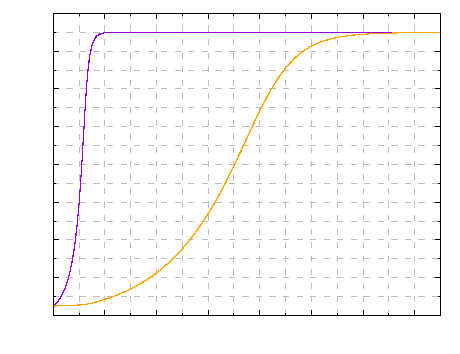
\includegraphics{2-bacteris}}%
    \gplfronttext
  \end{picture}%
\endgroup

	\caption{Evolution of the relative mass of the populations of mesophilic and thermophilic organisms}
	\label{fig:poblacions}
\end{figure}

\begin{figure}[htb]
	\sffamily \footnotesize \centering
	% GNUPLOT: LaTeX picture with Postscript
\begingroup
\newcommand{\etiqueta}[1]{\setlength{\fboxsep}{0.75pt}\colorbox{white}{#1}}
  \makeatletter
  \providecommand\color[2][]{%
    \GenericError{(gnuplot) \space\space\space\@spaces}{%
      Package color not loaded in conjunction with
      terminal option `colourtext'%
    }{See the gnuplot documentation for explanation.%
    }{Either use 'blacktext' in gnuplot or load the package
      color.sty in LaTeX.}%
    \renewcommand\color[2][]{}%
  }%
  \providecommand\includegraphics[2][]{%
    \GenericError{(gnuplot) \space\space\space\@spaces}{%
      Package graphicx or graphics not loaded%
    }{See the gnuplot documentation for explanation.%
    }{The gnuplot epslatex terminal needs graphicx.sty or graphics.sty.}%
    \renewcommand\includegraphics[2][]{}%
  }%
  \providecommand\rotatebox[2]{#2}%
  \@ifundefined{ifGPcolor}{%
    \newif\ifGPcolor
    \GPcolortrue
  }{}%
  \@ifundefined{ifGPblacktext}{%
    \newif\ifGPblacktext
    \GPblacktextfalse
  }{}%
  % define a \g@addto@macro without @ in the name:
  \let\gplgaddtomacro\g@addto@macro
  % define empty templates for all commands taking text:
  \gdef\gplbacktext{}%
  \gdef\gplfronttext{}%
  \makeatother
  \ifGPblacktext
    % no textcolor at all
    \def\colorrgb#1{}%
    \def\colorgray#1{}%
  \else
    % gray or color?
    \ifGPcolor
      \def\colorrgb#1{\color[rgb]{#1}}%
      \def\colorgray#1{\color[gray]{#1}}%
      \expandafter\def\csname LTw\endcsname{\color{white}}%
      \expandafter\def\csname LTb\endcsname{\color{black}}%
      \expandafter\def\csname LTa\endcsname{\color{black}}%
      \expandafter\def\csname LT0\endcsname{\color[rgb]{1,0,0}}%
      \expandafter\def\csname LT1\endcsname{\color[rgb]{0,1,0}}%
      \expandafter\def\csname LT2\endcsname{\color[rgb]{0,0,1}}%
      \expandafter\def\csname LT3\endcsname{\color[rgb]{1,0,1}}%
      \expandafter\def\csname LT4\endcsname{\color[rgb]{0,1,1}}%
      \expandafter\def\csname LT5\endcsname{\color[rgb]{1,1,0}}%
      \expandafter\def\csname LT6\endcsname{\color[rgb]{0,0,0}}%
      \expandafter\def\csname LT7\endcsname{\color[rgb]{1,0.3,0}}%
      \expandafter\def\csname LT8\endcsname{\color[rgb]{0.5,0.5,0.5}}%
    \else
      % gray
      \def\colorrgb#1{\color{black}}%
      \def\colorgray#1{\color[gray]{#1}}%
      \expandafter\def\csname LTw\endcsname{\color{white}}%
      \expandafter\def\csname LTb\endcsname{\color{black}}%
      \expandafter\def\csname LTa\endcsname{\color{black}}%
      \expandafter\def\csname LT0\endcsname{\color{black}}%
      \expandafter\def\csname LT1\endcsname{\color{black}}%
      \expandafter\def\csname LT2\endcsname{\color{black}}%
      \expandafter\def\csname LT3\endcsname{\color{black}}%
      \expandafter\def\csname LT4\endcsname{\color{black}}%
      \expandafter\def\csname LT5\endcsname{\color{black}}%
      \expandafter\def\csname LT6\endcsname{\color{black}}%
      \expandafter\def\csname LT7\endcsname{\color{black}}%
      \expandafter\def\csname LT8\endcsname{\color{black}}%
    \fi
  \fi
    \setlength{\unitlength}{0.0500bp}%
    \ifx\gptboxheight\undefined%
      \newlength{\gptboxheight}%
      \newlength{\gptboxwidth}%
      \newsavebox{\gptboxtext}%
    \fi%
    \setlength{\fboxrule}{0.5pt}%
    \setlength{\fboxsep}{1pt}%
\begin{picture}(4420.00,3400.00)%
    \gplgaddtomacro\gplbacktext{%
      \csname LTb\endcsname%%
      \put(487,380){\makebox(0,0)[r]{\strut{}\num{0}}}%
      \csname LTb\endcsname%%
      \put(487,743){\makebox(0,0)[r]{\strut{}\num{20}}}%
      \csname LTb\endcsname%%
      \put(487,1105){\makebox(0,0)[r]{\strut{}\num{40}}}%
      \csname LTb\endcsname%%
      \put(487,1468){\makebox(0,0)[r]{\strut{}\num{60}}}%
      \csname LTb\endcsname%%
      \put(487,1830){\makebox(0,0)[r]{\strut{}\num{80}}}%
      \csname LTb\endcsname%%
      \put(487,2193){\makebox(0,0)[r]{\strut{}\num{100}}}%
      \csname LTb\endcsname%%
      \put(487,2555){\makebox(0,0)[r]{\strut{}\num{120}}}%
      \csname LTb\endcsname%%
      \put(487,2918){\makebox(0,0)[r]{\strut{}\num{140}}}%
      \csname LTb\endcsname%%
      \put(487,3280){\makebox(0,0)[r]{\strut{}\num{160}}}%
      \csname LTb\endcsname%%
      \put(554,261){\makebox(0,0){\strut{}\num{0}}}%
      \csname LTb\endcsname%%
      \put(1077,261){\makebox(0,0){\strut{}\num{2}}}%
      \csname LTb\endcsname%%
      \put(1601,261){\makebox(0,0){\strut{}\num{4}}}%
      \csname LTb\endcsname%%
      \put(2124,261){\makebox(0,0){\strut{}\num{6}}}%
      \csname LTb\endcsname%%
      \put(2648,261){\makebox(0,0){\strut{}\num{8}}}%
      \csname LTb\endcsname%%
      \put(3171,261){\makebox(0,0){\strut{}\num{10}}}%
      \csname LTb\endcsname%%
      \put(3695,261){\makebox(0,0){\strut{}\num{12}}}%
      \csname LTb\endcsname%%
      \put(4218,261){\makebox(0,0){\strut{}\num{14}}}%
    }%
    \gplgaddtomacro\gplfronttext{%
      \csname LTb\endcsname%%
      \put(100,1830){\rotatebox{-270}{\makebox(0,0){\strut{}$\mathsfit P \ (\si{kW})$}}}%
      \csname LTb\endcsname%%
      \put(2386,83){\makebox(0,0){\strut{}$\mathsfit t \ (\si{days})$}}%
      \csname LTb\endcsname%%
      \put(1077,1830){\rotatebox{-87}{\makebox(0,0){\strut{}\etiqueta{\footnotesize Mesophiles}}}}%
      \csname LTb\endcsname%%
      \put(1863,688){\rotatebox{10}{\makebox(0,0){\strut{}\etiqueta{\footnotesize Thermophiles}}}}%
    }%
    \gplbacktext
    \put(0,0){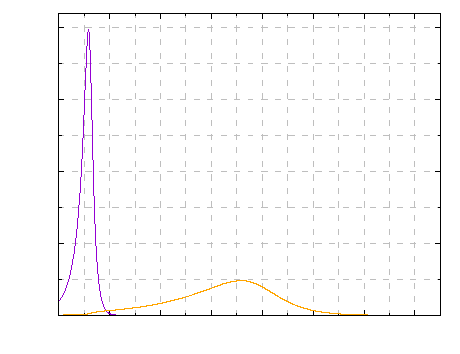
\includegraphics{2-potencies}}%
    \gplfronttext
  \end{picture}%
\endgroup

	\caption{Power output of the mesophilic and thermophilic reactions}
	\label{fig:potencies}
\end{figure}

\clearpage
\appendix
\section{References and Further Reading}
\begin{btSect}{fonts}
	\bibliographystyle{ieeetr}
	\subsection*{References}	
	\btPrintCited
\end{btSect}

\begin{btSect}{UphysicscNotes}
	\bibliographystyle{ieeetr}
	\subsection*{Further Reading}	
	\btPrintNotCited
\end{btSect}

\end{document}
